\section{Instant Messaging}

\frame{
  \frametitle{Inhaltsverzeichnis}
  \tableofcontents[currentsection]
}

\begin{frame}
  \frametitle{Übertragungsweg von Nachrichten}
  %\todo[inline]{Schaubild Übertragung von Nachrichten (über Server)}
  \center \inputSVG[\def\svgscale{0.25}]{Orange_blue_message_transportation_de}
  \todo[inline]{Farbe Pfeil ändern}
  \note{Analogie: Brief/Postkarte mit Adresse}
\end{frame}

\begin{frame}
  \frametitle{Symmetrische Verschlüsselung}
  \begin{columns}[c]
    \begin{column}{0.5\textwidth}
      \center \inputSVG[\def\svgscale{0.2}]{Orange_blue_symmetric_cryptography_de}
    \end{column}
  \end{columns}
  \todo[inline]{Schaubild Verschlüsselung (symm)}
\end{frame}

\begin{frame}
  \frametitle{Transportwegverschlüsselung / Ende-zu-Ende Verschlüsselung}
  Transportwegverschlüsselung
  \begin{center}
    \inputSVG[\def\svgscale{0.25}]{Orange_blue_message_transportation_security_de}
  \end{center}


  Ende-zu-Ende Verschlüsselung
  \center \inputSVG[\def\svgscale{0.25}]{Orange_blue_message_end_to_end_de}
%  \todo[inline]{Schaubild vgl. Ende-zu-Ende / Transportweg}
\end{frame}

\begin{frame}
  \frametitle{Transportweg- und Ende-zu-Ende Verschlüsselung}
  \todo[inline]{Ende-zu-Ende + Transportweg}
\end{frame}

\begin{frame}
  \frametitle{Open Source vs. Closed Source}
  \begin{definition}[Open Source]
   Programm mit öffentlich zugänglichem Quellcode \hfill \tiny [Duden]
  \end{definition}

  \begin{itemize}
   \item Programm kann von jedem geprüft werden
   \item Schwer Hintertüren einzubauen
   \item Notwenige Bedingung für prüfbar sichere Programme
   \item Open Source $\neq$ kostenlos
  \end{itemize}

\end{frame}


\begin{frame}
  \frametitle{EFF Scorecard zu Messaging Apps}
  \center
  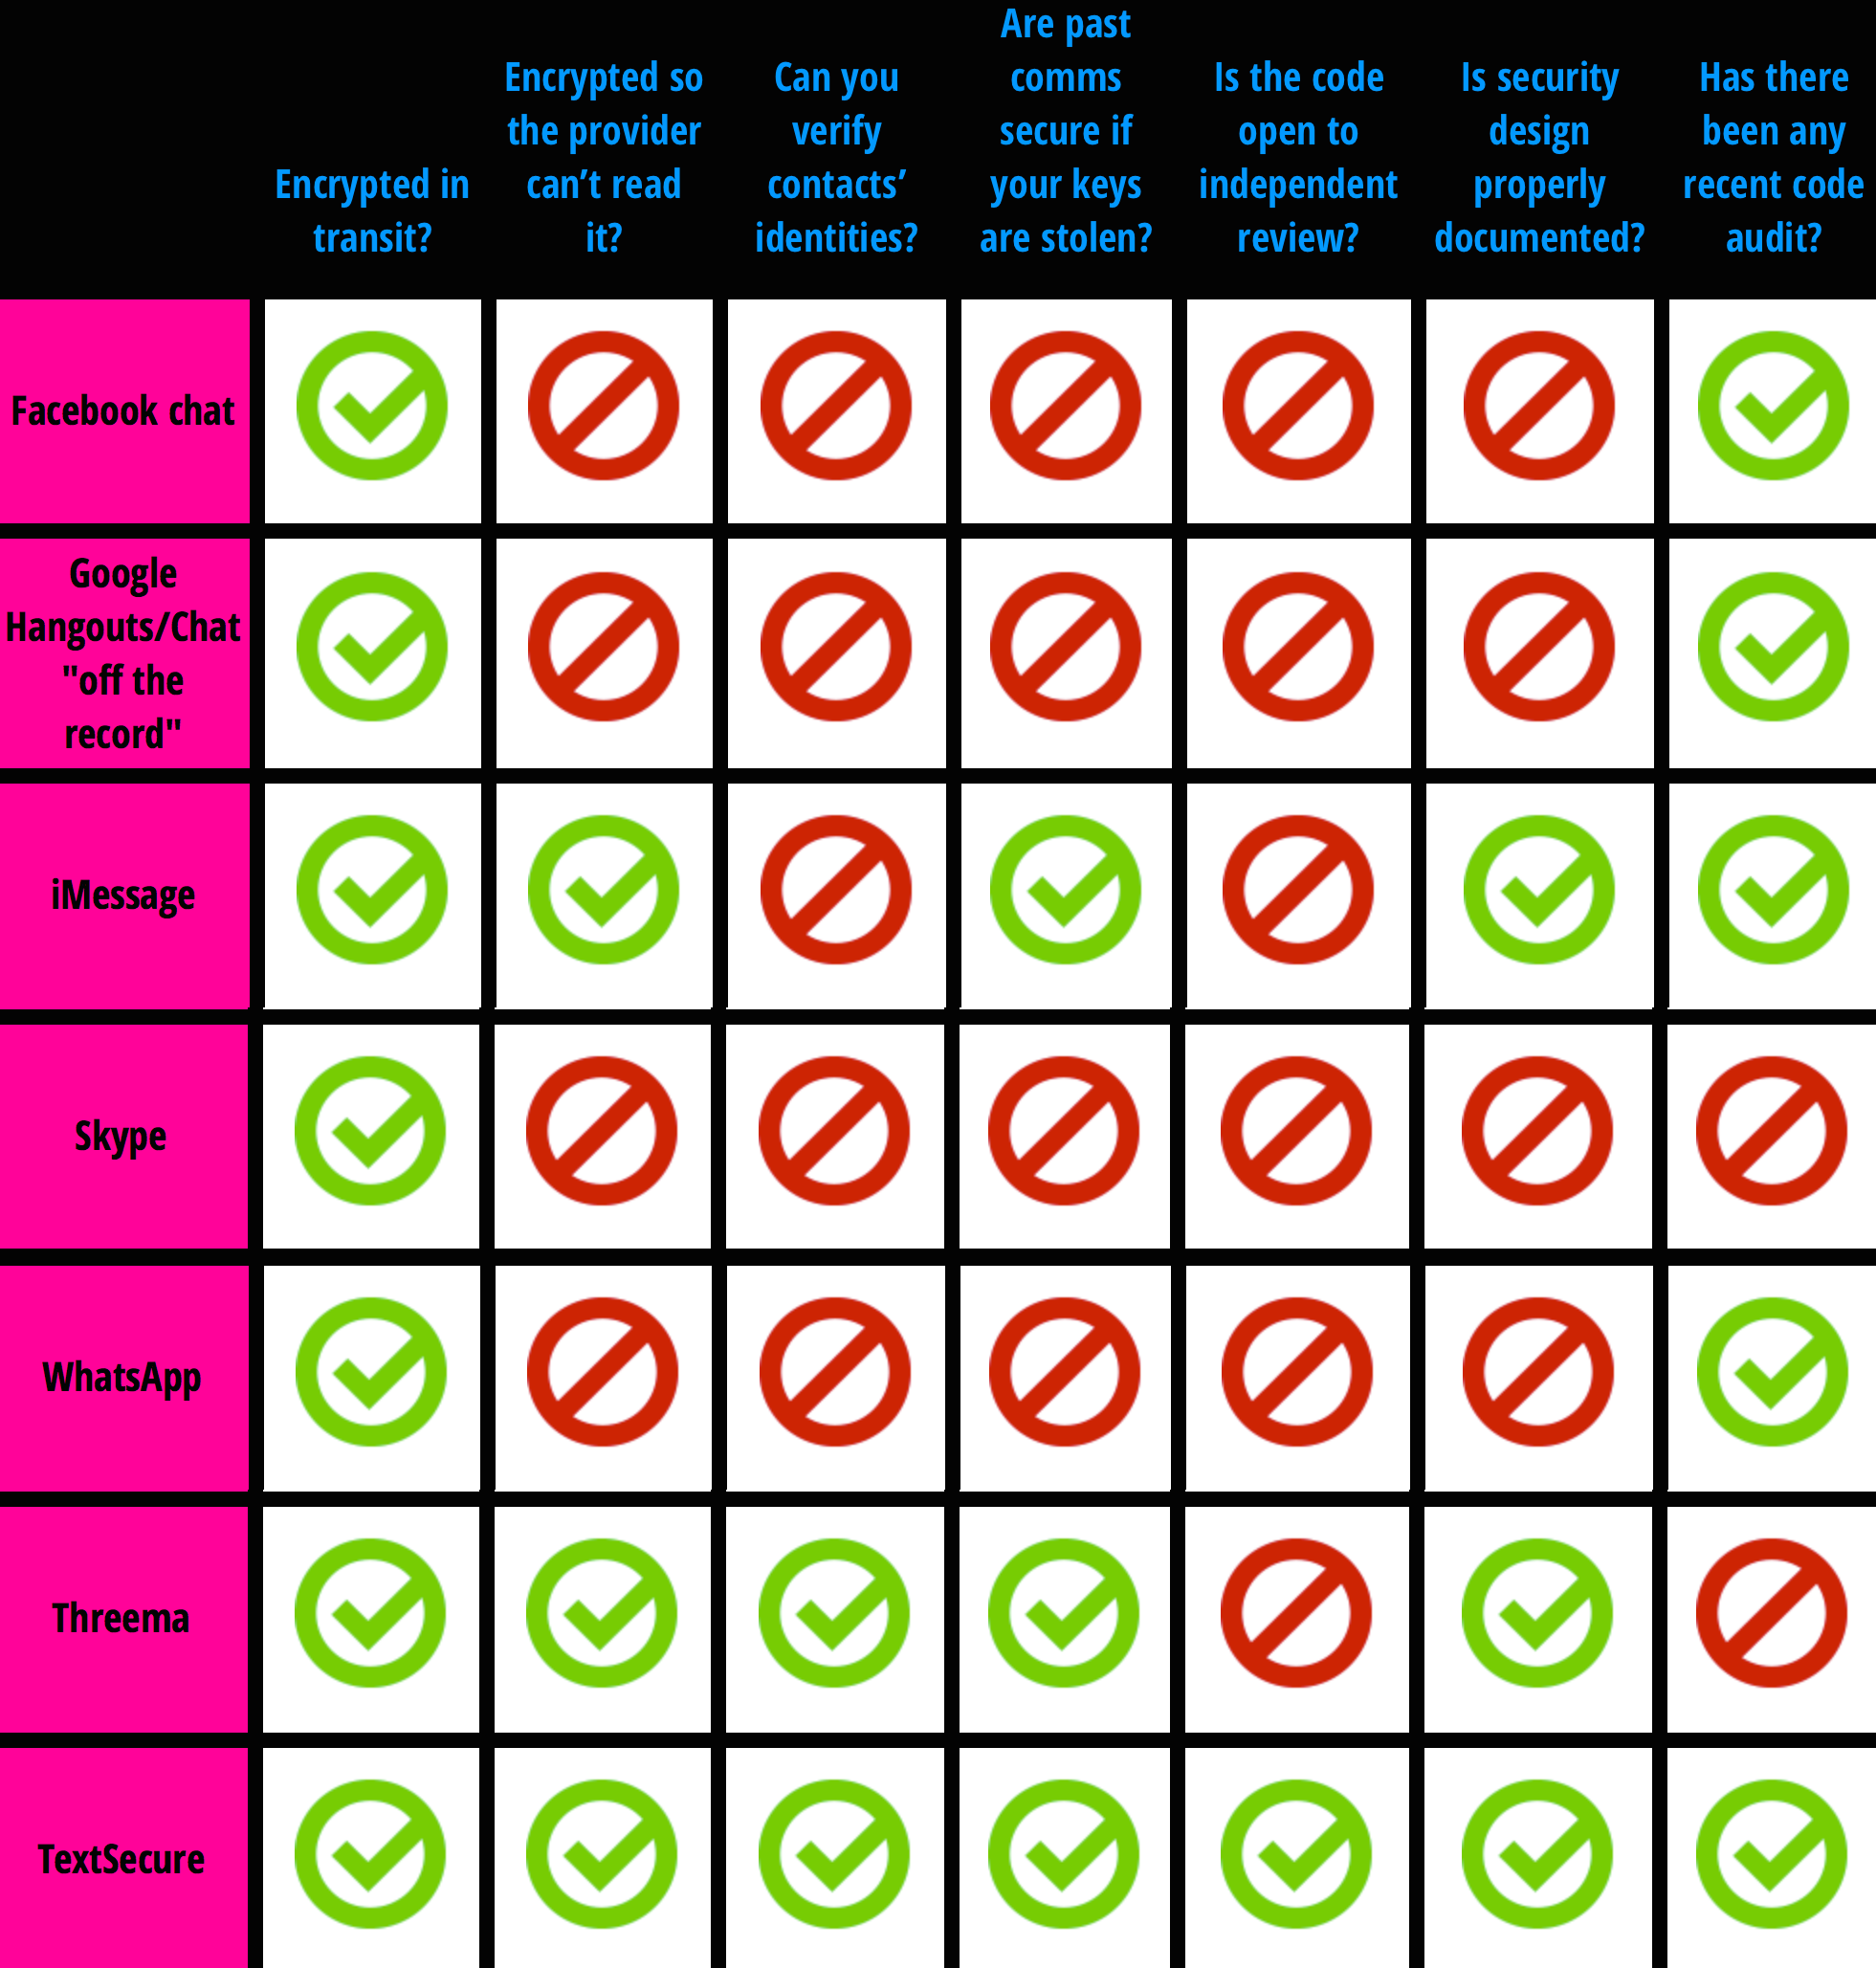
\includegraphics[width=0.6\textwidth]{figures/eff_scorecard.png}
\end{frame}

\begin{frame}
  \frametitle{Identitätsprüfung}
  \todo[inline]{Screenshots}
\end{frame}
